% Chapter fragment. Required packages in the main document:
% \usepackage{booktabs,graphicx,tabularx}

\chapter{Automatic land-cover classification}
\label{chap:classification}

The original practical provides the baseline classification. Its national
Random Forest uses the ten 2025 Sentinel-2 reflectance bands, 500 trees and a
minimum node size of 10. Recoded reference observations are divided by a
reproducible random 80/20 split; prediction is performed over the full raster
before cropping to the study area. This model reports 60.6\% overall accuracy
and 54.9\% balanced accuracy for its national test sample. These values are not
directly comparable with the later local results because the national random
split can place neighbouring observations in both subsets. Figure~\ref{fig:rf-map}(a)
shows the original national output cropped to Bregaglia.

The extensions retain the original class recoding and 100-m grid, but add five
spectral indices, seven DHM25 terrain variables, class weighting and parameter
tuning. Five-kilometre spatial blocks replace the random split; four folds are
used for selection and 367 observations in a fifth fold remain untouched. On
this common Bregaglia holdout, the raw national model reaches 62.9\% overall
and 61.8\% balanced accuracy, while the local terrain model reaches 67.8\% and
65.9\%. A hybrid improves balanced accuracy by only 0.3 percentage points, so
the local model is retained. Aggregating its nine predicted classes into six
groups raises the scores to 78.2\% and 76.3\%. This does not refit the model:
within-group confusions are simply no longer counted as errors.

Forest on the valley slopes and bare or glaciated surfaces at high elevation
are convincing relative to the natural-colour image. Open forest and river
were least reliable in the detailed output (38.1\% and 36.8\% F1). After
aggregation, forest reached 84.0\% F1, but water remained uncertain at 60.5\%,
especially along narrow rivers; isolated built-up pixels also require caution.
Sentinel-2 records physical surface properties, while some labels describe land
use that one image cannot resolve. A 100-m cell may also mix vegetation,
buildings, roads and water. Apparent boundaries should therefore be checked
against the satellite image, aerial imagery or local knowledge.

As an additional consistency check, the two detailed classifications were
compared with SSP1-2025 after nearest-neighbour projection to the same 100-m
grid. This is not an independent accuracy assessment: SSP1-2025 is another
model product, and disagreement may originate from either map. Across 33,905
paired cells, agreement increased from 51.0\% for the national Random Forest to
54.9\% for the local terrain model; balanced agreement increased from 36.8\%
to 40.1\%, and macro-IoU from 20.0\% to 22.4\%. Approximately 15.6\% of SSP1
cells belong to classes unavailable to the classifiers, principally
overgrown/shrubland. Restricting the comparison to supported SSP1 classes gives
60.5\% agreement for the national model and 65.1\% for the local model. Static,
closed forest and lake show the strongest spatial correspondence, whereas
open forest, river and artificial surfaces remain weak. These results support
the relative improvement of the local model but do not replace the reserved
reference-point assessment.

\clearpage
\section*{Tables and figures}

\begin{table}[!htbp]
  \centering
  \caption{Performance from the original national workflow and the subsequent
  Bregaglia extensions. The first row uses the original national random test;
  all remaining rows use the same Bregaglia spatial holdout. The first-row
  macro-F1 was reconstructed from the reported confusion matrix because the
  original workflow did not calculate it explicitly.}
  \label{tab:rf-model-comparison}
  \scriptsize
  \setlength{\tabcolsep}{3pt}
  \begin{tabularx}{\textwidth}{@{}p{0.14\textwidth}XXcccc@{}}
    \toprule
    Output and evaluation & Data sources and training scope & RF modelling choices & $K$ & OA (\%) & BA (\%) & F1 (\%) \\
    \midrule
    Original national model; random national test
      & Swiss AS\_27 reference points; ten 2025 Sentinel-2 bands; national 80/20 split
      & 500 trees; minimum node size 10; unweighted; untuned
      & 11 & 60.6 & 54.9 & 56.2 \\
    National transfer; raw Bregaglia spatial test
      & Swiss AS\_27 points outside Bregaglia, capped at 5,000 per class ($n=45{,}000$); ten bands
      & 500 trees; minimum node size 10; unweighted; untuned; evaluated on the untouched Bregaglia block fold
      & 9 & 62.9 & 61.8 & 60.2 \\
    Local terrain model; raw Bregaglia spatial test
      & Bregaglia AS\_27 points; ten bands, five indices and seven DHM25 terrain variables
      & Inverse-frequency class weights; 5-km blocks; four-fold tuning of \texttt{mtry}, node size, sampling fraction and split rule; 1,000-tree assessment model
      & 9 & 67.8 & 65.9 & 65.2 \\
    Hybrid national--local model; raw Bregaglia spatial test
      & National sample plus Bregaglia development blocks; bands, indices and terrain ($n=46{,}329$)
      & Inverse class weights; local cases weighted $5\times$; tuned settings; 1,000 trees
      & 9 & 68.9 & 66.2 & 65.3 \\
    Local post-hoc aggregation
      & Predictions from the fitted nine-class local terrain model
      & No new RF: related predictions and reference labels merged from nine to six classes before scoring
      & 6 & \textbf{78.2} & \textbf{76.3} & \textbf{75.7} \\
    Local direct coarse retraining
      & Same Bregaglia predictors; reference labels merged to six classes before fitting
      & Inverse class weights; block cross-validation and tuning repeated for six classes; 1,000 trees
      & 6 & 76.6 & 72.8 & 73.1 \\
    \bottomrule
  \end{tabularx}
\end{table}

\begin{table}[!htbp]
  \centering
  \caption{Cross-model agreement with SSP1-2025 on 33,905 paired Bregaglia
  cells. These are consistency measures, not validation accuracies.}
  \label{tab:ssp1-agreement-summary}
  \small
  \setlength{\tabcolsep}{4pt}
  \resizebox{\textwidth}{!}{%
  \begin{tabular}{lrrrrrr}
    \toprule
    RF output & Overall agreement (\%) & Balanced agreement (\%) & Macro-IoU (\%) & $\kappa$ & Unsupported (\%) & Supported-only agreement (\%) \\
    \midrule
    National RF      & 51.0 & 36.8 & 20.0 & 0.389 & 15.6 & 60.5 \\
    Local terrain RF & 54.9 & 40.1 & 22.4 & 0.429 & 15.7 & 65.1 \\
    \bottomrule
  \end{tabular}
  }
\end{table}

\begin{table}[!htbp]
  \centering
  \caption{Class-wise intersection over union with SSP1-2025. Zero values
  identify classes absent from the corresponding Random Forest output.}
  \label{tab:ssp1-class-iou}
  \small
  \begin{tabular}{lrr@{\qquad}lrr}
    \toprule
    Class & National & Local & Class & National & Local \\
          & IoU (\%) & IoU (\%) & & IoU (\%) & IoU (\%) \\
    \midrule
    Urban/amenities      & 1.6  & 7.3  & Alpine pastures      & 42.4 & 42.0 \\
    Static               & 54.0 & 57.8 & Grassland or meadows & 17.7 & 24.2 \\
    Open Forest          & 5.5  & 10.8 & Permanent crops      & 0.2  & 0.0 \\
    Closed forest        & 45.0 & 46.8 & Glacier              & 19.0 & 21.1 \\
    Overgrown/shrubland  & 0.0  & 0.0  & Lake                 & 52.3 & 55.5 \\
    Agriculture          & 0.0  & 0.0  & River                & 2.6  & 3.2 \\
    \bottomrule
  \end{tabular}
\end{table}

\begin{table}[!htbp]
  \centering
  \caption{Class-level F1 scores after aggregation to the mapped six-class
  scheme.}
  \label{tab:rf-class-performance}
  \small
  \begin{tabular}{lrrrrrr}
    \toprule
    Class & Artificial & Static/bare & Forest & Grassland & Glacier/snow & Water \\
    \midrule
    F1 (\%) & 72.4 & 83.2 & 84.0 & 72.1 & 81.8 & 60.5 \\
    \bottomrule
  \end{tabular}
\end{table}

\begin{figure}[!htbp]
  \centering
  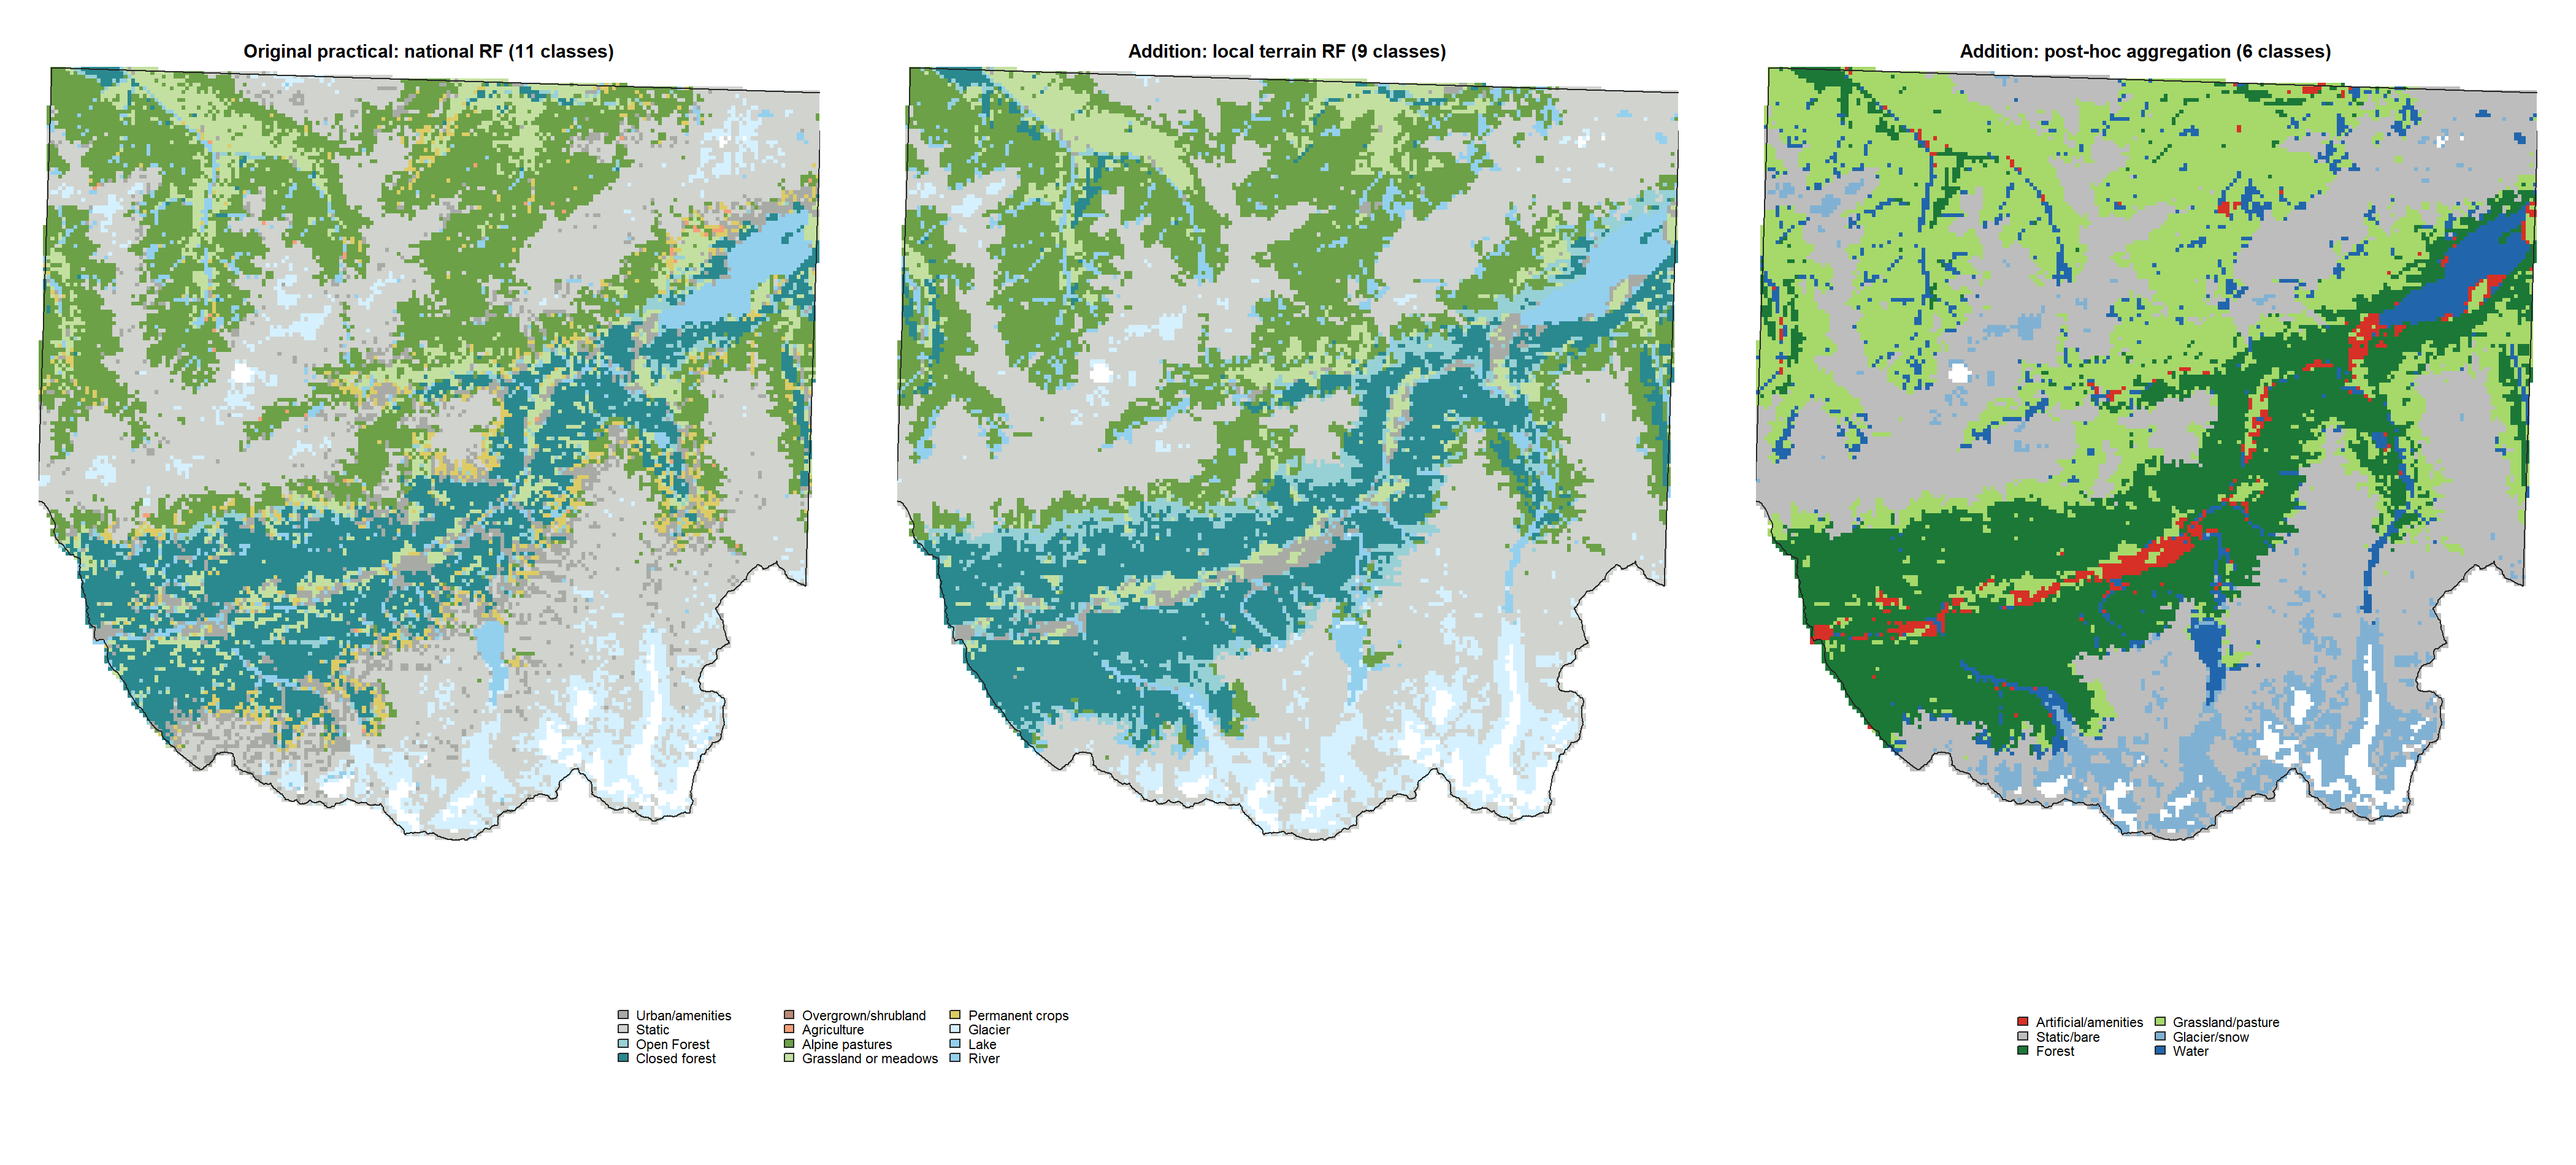
\includegraphics[width=0.99\textwidth]{figures/chapter2_rf_bregaglia_2025_baseline_and_additions.png}
  \caption{Land-cover predictions for Bregaglia in 2025. (a) Original national
  ten-band Random Forest cropped to the commune; 11 detailed SSP-CH classes are
  predicted. (b) Extended local Random Forest using bands, indices and terrain;
  nine classes are predicted because agriculture and permanent crops are
  locally rare and shrubland lacks an exclusive reference group. (c) The same
  local predictions aggregated after classification to six classes. White
  cells lacked a complete predictor set and were not classified.}
  \label{fig:rf-map}
\end{figure}

\begin{figure}[!htbp]
  \centering
  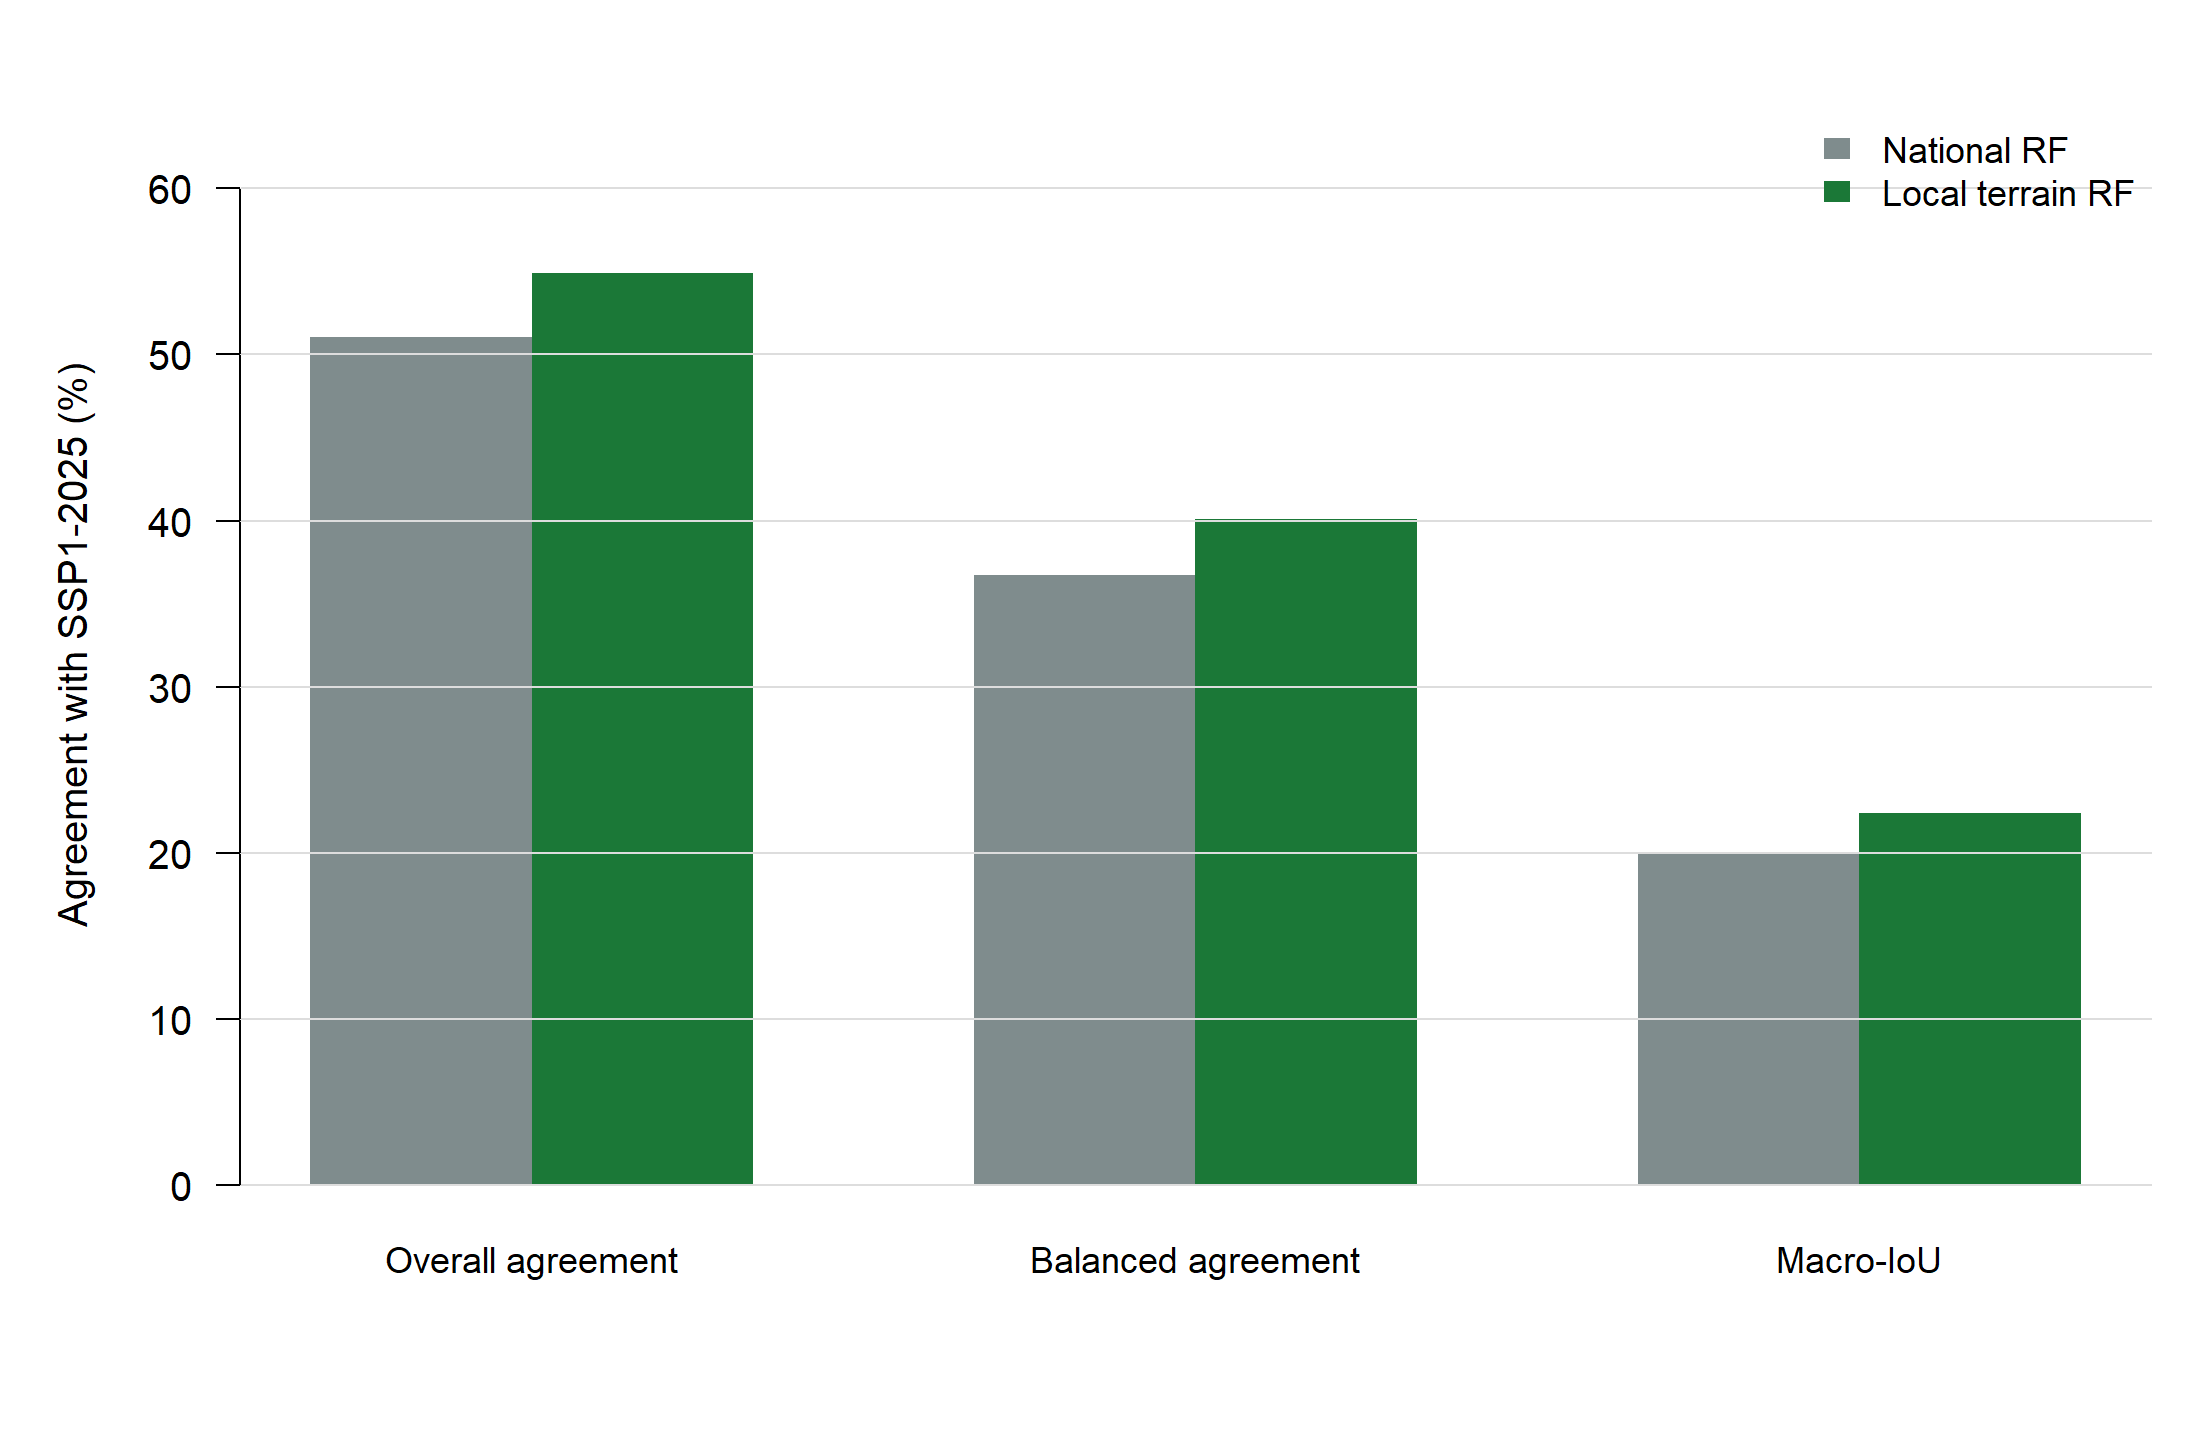
\includegraphics[width=0.82\textwidth]{figures/ssp1_2025_rf_agreement_summary.png}
  \caption{Overall, balanced and macro-IoU agreement of the national and local
  Random Forest outputs with SSP1-2025. The consistently higher local values
  indicate improved cross-model correspondence, not independent accuracy.}
  \label{fig:ssp1-agreement-summary}
\end{figure}

\begin{figure}[!htbp]
  \centering
  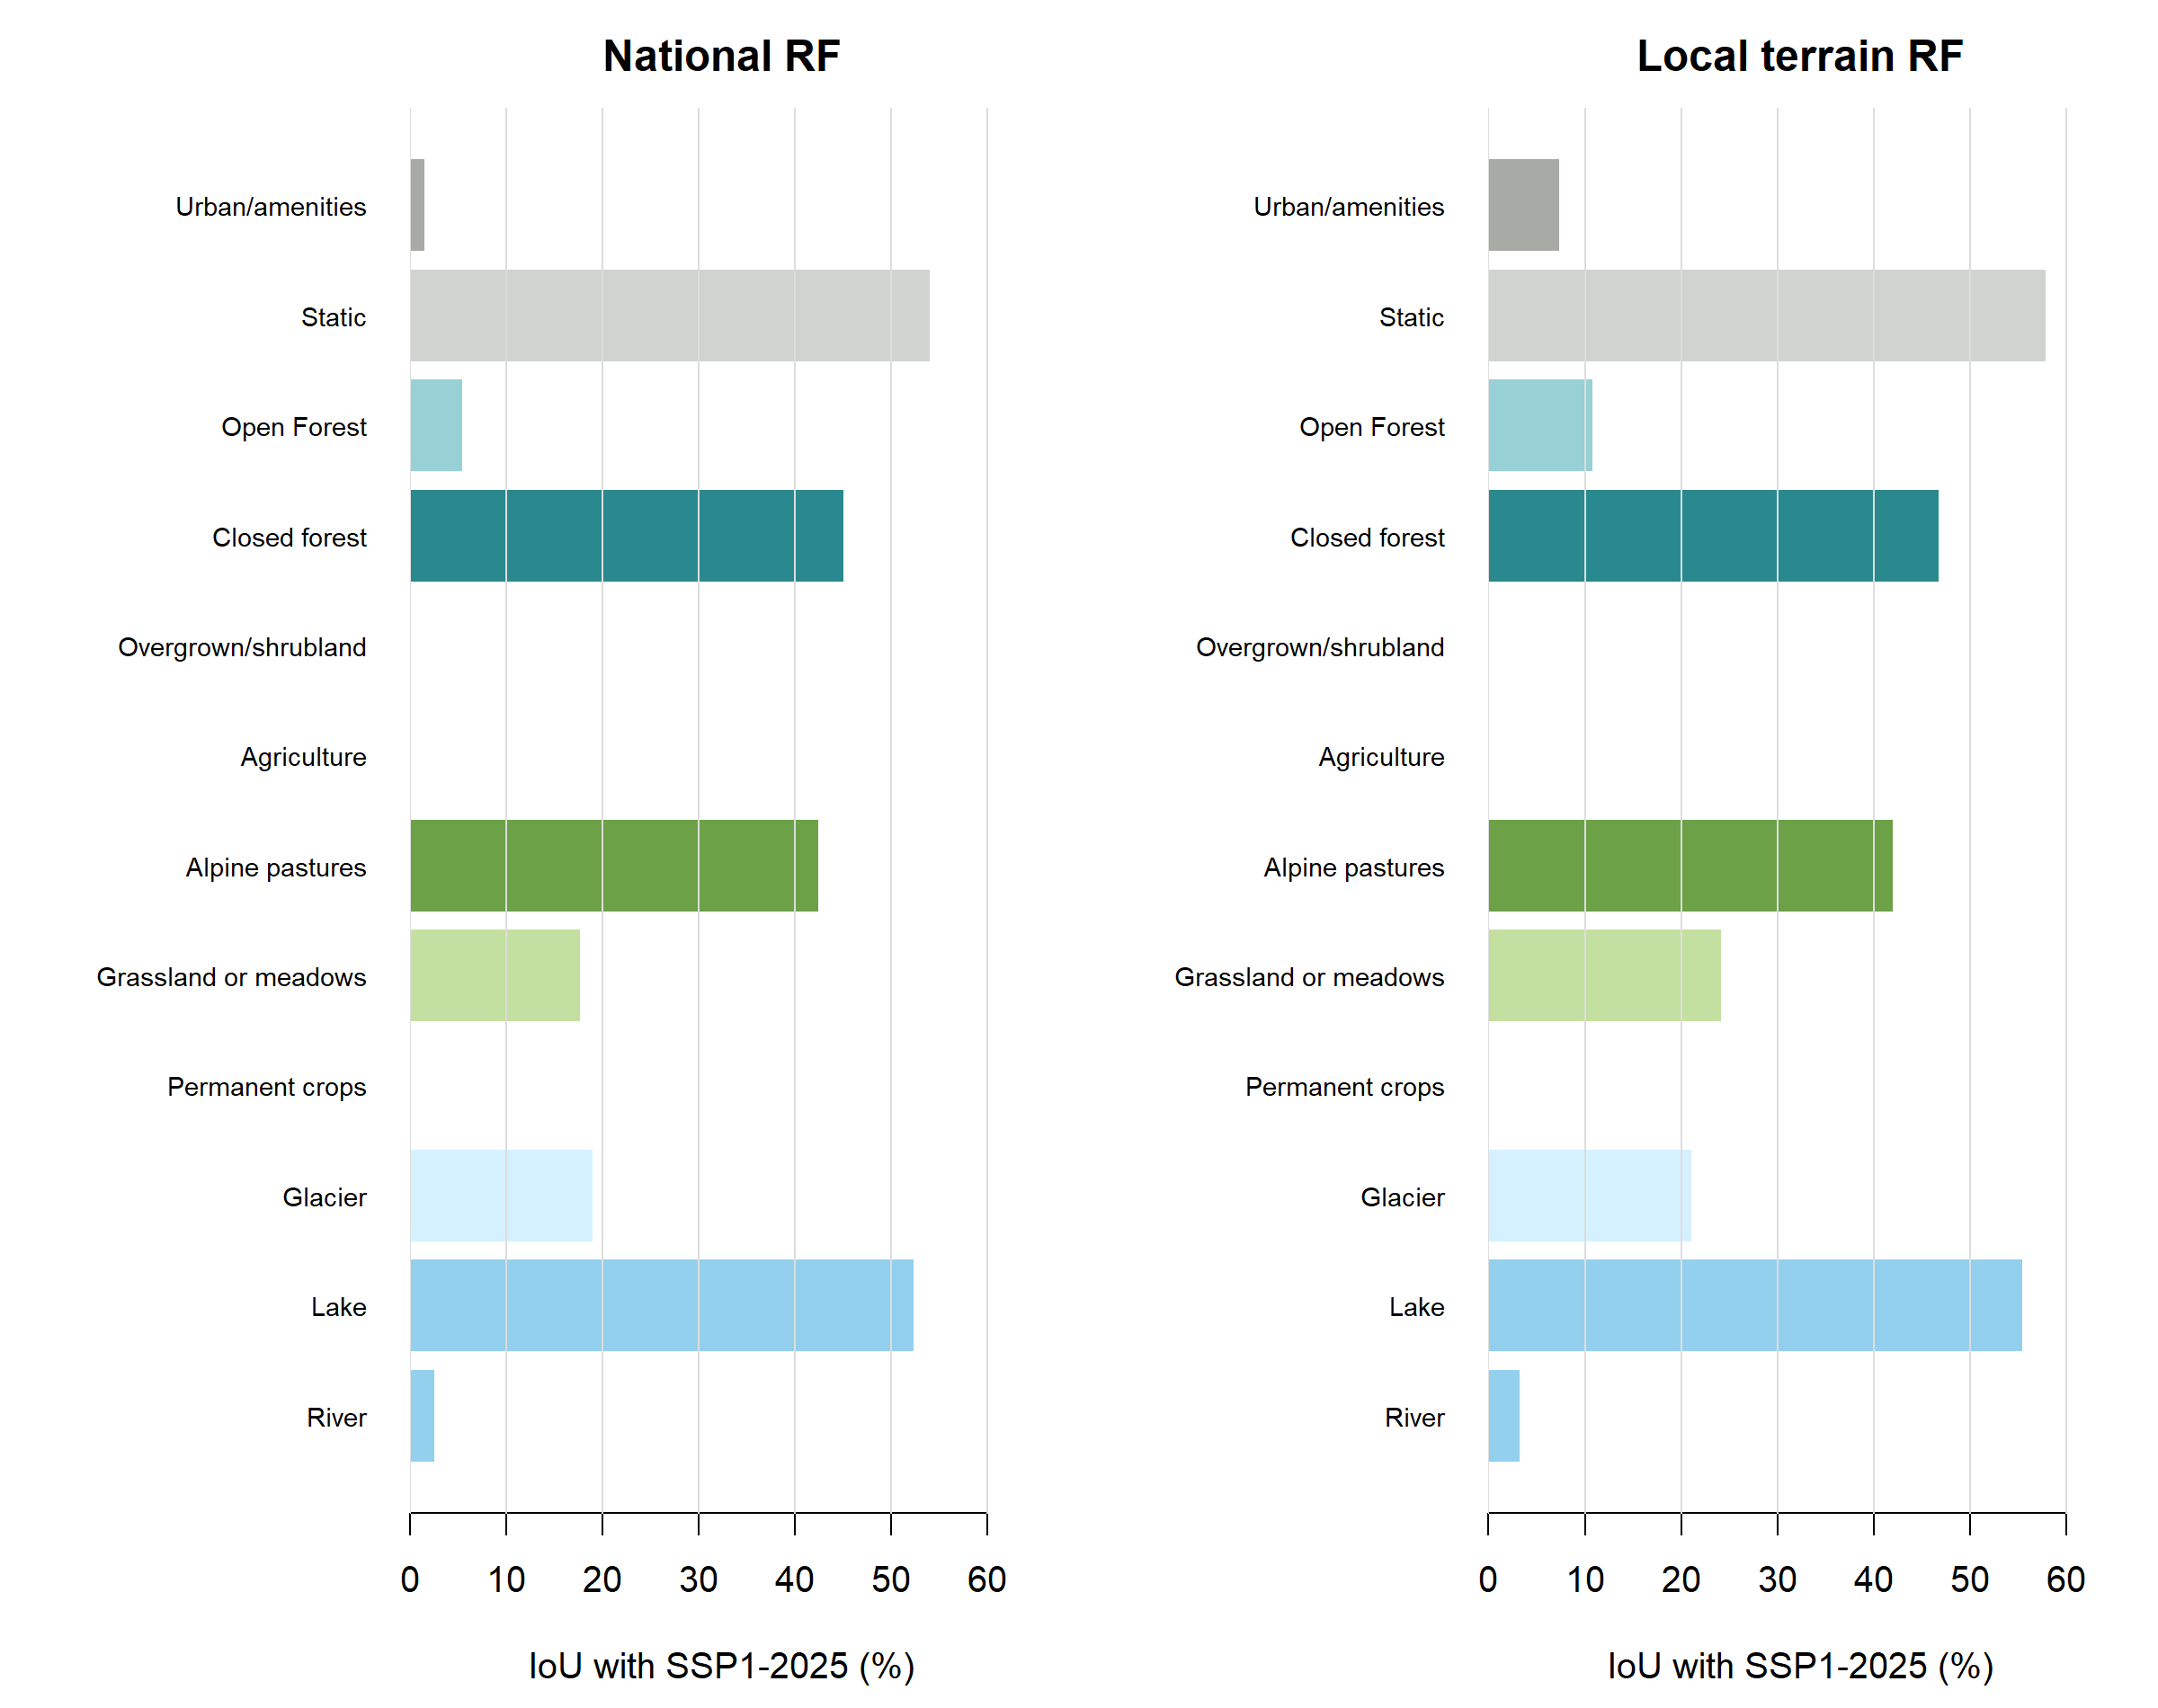
\includegraphics[width=0.94\textwidth]{figures/ssp1_2025_rf_class_iou.png}
  \caption{Class-wise IoU with SSP1-2025 for the national and local Random
  Forest outputs. Class colours match those used for the SSP-CH scenario maps;
  both panels use the same horizontal scale.}
  \label{fig:ssp1-class-iou}
\end{figure}

